\chapter{Observing Falling Filters}

	\begin{quotation}
		\textit{The ability to observe without evaluating is the highest form of intelligence.} \sourceatright{Jiddu Krishnamurti}
	\end{quotation}

While Mr.\ Krishnamuri may be making a stretch with his superlative, it remains true that observing without evaluating is essential for the creation of knowledge.
In our lives, we have bias (conceptions, self-constructed mental models) that we use as our lens to view the world.
These models are based on how each of us were socialized and on our subsequent experience.
To learn and create new knowledge, we must develop skill in observation.
In this lab, we will direct you to make detailed, careful quantitative observations, describe the patterns you find with mathematics, and finally make some wild guesses (``hypotheses'') about a more universal principle that explains this pattern that one could use to make predictions.
Due to time and brain constraints, we will not, in this lab, test those hypotheses.

\section*{Learning Goals}

 \begin{itemize}

  \item Conduct an observation experiment, including collecting data, finding and describing a pattern quantitatively, including presentation of data graphically and formulating a quantitative hypothesis.

  \item Use measurement uncertainty to describe physical quantities meaningfully.
  
  \item Format a lab report in a helpful way.
 \end{itemize}

\section*{The Scientific Cycle\protect\footnote{adapted from \cite{etkina_college_2014}}}

Astrophysics is an experimental science. To answer questions, astrophysicists do not just think and dream in their offices but constantly engage in experimental investigations. Astrophysicists use special measuring devices to observe phenomena (natural and planned), describe their observations (carefully record them using words, numbers, graphs, etc.), find repeating features called patterns (for example, the distance traveled by a falling object is directly proportional to the square of the time of flight), and then try to explain these patterns. By doing this, astrophysicists describe and answer the questions of ``why'' or ``how'' the phenomena happened and then deduce quantitative rules called mathematical models that explain the phenomena.

However, a deduced explanation or a mathematical model is not automatically accepted as true. Every model needs to undergo careful testing. When astrophysicists test a model, they use the model to predict the outcomes of new experiments. As long as there is no experiment whose outcome is inconsistent with predictions made using the model, it is not disproved. However, a new experiment could be devised tomorrow whose outcome is not consistent with the prediction made using the model. The point is that there is no way to ``prove'' a model once and for all. At best, the model just hasn't been disproven yet.

A simple example will help you understand some processes that physicists follow when they study the world. One model for the scientific process will also be described (there are other helpful models, and there is no one true ``scientific method''). Imagine that you walk into the house of your acquaintance Bob and see 10 tennis rackets of different quality and sizes. This is an \textbf{observational experiment}. During an observational experiment, a scientist collects data that seem important. Sometimes it is an accidental or unplanned experiment. The scientist has no prior expectation of the outcome. In this case, the number of tennis rackets and their quality and sizes represent the data. Having so many tennis rackets seems unusual to you, so you try to explain the data you collected (or, in other words, to explain why Bob has so many rackets) by devising several hypotheses. A \textbf{hypothesis} is an explanation that usually is based on some mechanism that is behind what is going on, or it can be a mathematical model describing the phenomenon. One hypothesis is that Bob has lots of children and they all play tennis. A second hypothesis is that Bob makes his living by fixing tennis rackets. A third hypothesis is that he is a thief who steals tennis rackets.

How do you decide which hypothesis is correct? You may reason: if Bob has many children who play tennis, and I walk around the house checking the sizes of clothes that I find, then I will find clothes of different sizes. Checking the clothing sizes is a new experiment, called a \textbf{testing experiment}. A testing experiment is different from an observational experiment. In a testing experiment, a specific hypothesis is being ``put on trial.'' This hypothesis is used to construct a clear expectation of the outcome of the experiment. This clear expectation (based on the hypothesis being tested) is called a \textbf{prediction}. So you conduct the testing experiment by walking around the house checking the closets. You do find clothes of different sizes. This is the \textbf{outcome} of your testing experiment. Does it mean for absolute certain that Bob has the rackets because all of his children play tennis? No; he could still be a racket repairman or a thief. Therefore, if the outcome of the testing experiment matches the prediction based on your hypothesis, you cannot say that you proved the hypothesis. All you can say is that you failed to disprove it. However, if you walk around the house and do not find any children's clothes, you can say with more confidence that the number of rackets in the house is not due to Bob having lots of children who play tennis. Still, this conclusion would only be valid if you made an \textbf{assumption}: Bob's children live in the house and wear clothes of different sizes. Generally, in order to reject a hypothesis, you need to check the additional assumptions you made and determine if they are reasonable.

Imagine you have rejected the first hypothesis (you didn't find any children's clothes). Next, you wish to test the hypothesis that Bob is a thief. This is your reasoning: \textit{If} Bob is a thief (the hypothesis), \textit{and} I walk around the house checking every drawer (the testing experiment), \textit{then} I will not find any receipts for the tennis rackets (the prediction). You perform the experiment and you find no receipts. Does it mean that Bob is a thief? He might just be a disorganized father of many children or a busy repairperson. However, if you find all the receipts, you can say with more confidence that he is not a thief (but he could still be a repairperson). Thus it is possible to disprove (rule out) a hypothesis, but it is not possible to prove it once and for all. The process that you went through to create and test your hypothesis is depicted in Figure~\ref{me:fig:isle}. At the end of your investigation you might be left with a hypothesis that you failed to disprove. As an astrophysicist you would now have some confidence in this hypothesis and start using it for practical applications, or \textbf{application experiments}.

\begin{figure}
	\centering
	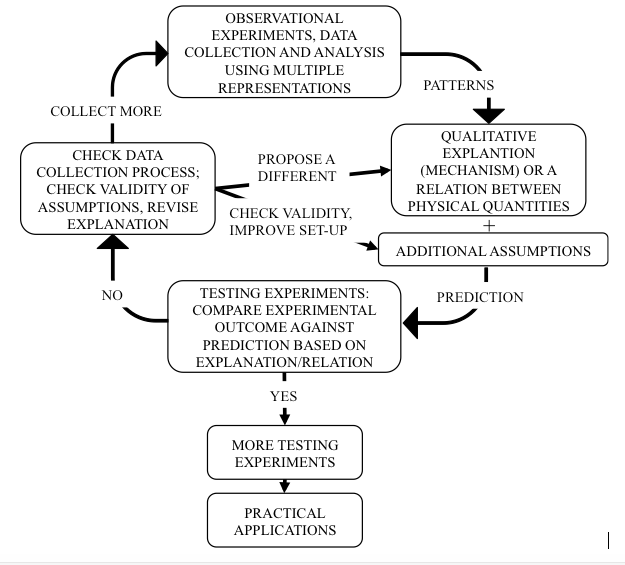
\includegraphics[width=0.7\textwidth]{measurement/islegraphic.png}
	\caption{A model of the process some scientists go through to create knowledge.\cite{etkina_millikan_2015}}\label{me:fig:isle}
\end{figure}

% ideas: measure cotton balls, rocks, rigid objects with finger, ruler, caliper; discover pi with various circles; quantify using popcorn popper and distance; everyone measures the same thing repeatedly, build up a normal distribution; dropping a needle on a lined paper repeatedly to get something like pi.
 
% pieces: Sci Ab rubrics B, G, F; measurement uncertainty terminology, practice handout

%\section*{Premise}

%\textbf{Premise:} In large competitive engineering grants and awards, for example Google Lunar X-Prize, teams must complete milestones by certain deadlines to stay in the race, so that they justify being granted continued resources for the next stages. In our imaginary situation, you are competing for the Barker X-Prize, to push the envelope of Galilean mechanics to address the question, ``do objects really fall at the same rate? If not, what affects this?'' Team performance will be compared with other teams at each stage.

\section*{Today's lab}

In today's lab, you will investigate the relationship between the size of coffee filters and how long it takes them to fall. In the first section, you will determine the size of the coffee filters. In the second, you will determine how long each take to fall, controlling for other variables, and then find a mathematical pattern that describes the relationship.

\section{Application experiment: how big are the filters?}

\textbf{Goal:} Find the cross-sectional area of each coffee filter using two different methods and make a final determination of that area, including uncertainty in that area, for use in the next experiment.
%In Stage 1 of the Barker X-Prize, each team has been tasked with determining precisely how big various objects are, including marbles, cotton balls, and coffee filters, including a detailed determination of their uncertainty of these measurements.
 
\textbf{Available equipment:} several differently-sized coffee filters, meter stick, camera (on your phone), Computer with ImageJ installed, string

\begin{framed}
	ImageJ is an image analysis program that includes, among other things, the ability to measure lengths, angles, and areas in images, provided that you give it a scale for how long some reference object is in the image.
\end{framed}

\begin{enumerate}
	\item You may want to decide on roles for each group member. Example roles include Facilitator (ensures time and group focus are efficiently used), Scribe (ensures work is recorded), Technician (oversees apparatus assembly, usage), Skeptic (ensures group is questioning itself). Note that each role is responsible for ensuring that the thing happens, rather than necessarily doing it themselves.
	
	\item Review Rubrics D and G and discuss any unclear expectations with your group and the instructor.
	
	\item Discuss with your group what cross-sectional area means and why it might affect the fall time.
	
	\item Brainstorm different methods to measure the cross-sectional area. Come up with two independent methods for determining the cross-sectional area. The purpose is that if you make a mistake or wrong assumption in one method, then the method (hopefully) gives a different result than the other method. For discovering new things, this is one quantitative way of checking your work, since you don't have the answer ahead of time.
	
	\item Discuss with an instructor your two methods before you begin. They will help increase the chances that your method will lead to successful results, or at least that the unhelpful path that you choose will take a short enough amount of time for you to change it when you discover it does not work. We want you to have productive failure that you have time to learn from.
	
	\item For each method,
	\begin{enumerate}
		\item Agree on a procedure and collect the data.
	\end{enumerate}
	
\end{enumerate}
 
\section{how things fall}

%Rationale:
%\begin{enumerate}
% \item want one experiment where students measure lengths and estimate uncertainties that are needed for data analysis. Lengths are intuitive things for students, no prior teaching needed. Then they see how those lengths compare to something else in a physics-y way. Then they graph it and decide what functions might describe them.
 
% \item falling and air resistance is good here. air resistance depends on cross sectional area, so length measurement. Data is not simple and obvious, but is instead messy, making pattern identification non-trivial, but still possible. Also cannot just use or look-up simple answers online -> authentic inquiry.
 
% \item so could do area vs. time to hit the floor. Can measure with video tracking, photogates, motion detector, stopwatch. need multiple sizes of coffee filters.
 
% \item Or position vs. time for different objects. This should give some interesting graphs, since objects can vary from no-meaningful-air-resistance to dominated-by-air-resistance constant. And the latter case should have an acceleration at the beginning, then constant, so it's more complicated. Must use video tracking or motion detection. So includes the skill of choosing with data to model. is there one function that works for all parts, or is there a transition between different situations?
 
% \item for video tracking, need to know how students can find framerate of videos they take, make sure it's easily imported to OSP Tracker.
%\end{enumerate}

Steps:
\begin{enumerate}
 \item Identify the phenomemon to be investigated.
 
 \item Design a reliable experiment that investigates the phenomenon.
 
 \item Decide what physical quantities are to be measured and identify independent and dependent variables.
 
 \item Describe how to use available equipment to make measurements.
 
 \item 
\end{enumerate}

\section{If in Stars class, also do this:}

15 minutes before end of lab, introduce H-R diagram lab.

Submit observation to queue

\section{Post-lab survey}

[Include Anna Karelina's flow questions here]